%%%%%%%%%%%%%%%%%%%%%%%%%%%%%%%%%%%%%%%%%
% Programming/Coding Assignment
% LaTeX Template
%
% This template has been downloaded from:
% http://www.latextemplates.com
%
% Original author:
% Ted Pavlic (http://www.tedpavlic.com)
%
% Note:
% The \lipsum[#] commands throughout this template generate dummy text
% to fill the template out. These commands should all be removed when 
% writing assignment content.
%
% This template uses a Perl script as an example snippet of code, most other
% languages are also usable. Configure them in the "CODE INCLUSION 
% CONFIGURATION" section.
%
%%%%%%%%%%%%%%%%%%%%%%%%%%%%%%%%%%%%%%%%%

%----------------------------------------------------------------------------------------
%	PACKAGES AND OTHER DOCUMENT CONFIGURATIONS
%----------------------------------------------------------------------------------------

\documentclass{article}
\usepackage[english]{babel}
\usepackage{amsmath}
\usepackage{fancyhdr} % Required for custom headers
\usepackage{lastpage} % Required to determine the last page for the footer
\usepackage{extramarks} % Required for headers and footers
\usepackage[usenames,dvipsnames]{color} % Required for custom colors
\usepackage{graphicx} % Required to insert images
\usepackage{subcaption}
\usepackage{listings} % Required for insertion of code
\usepackage{courier} % Required for the courier font
\usepackage{lipsum} % Used for inserting dummy 'Lorem ipsum' text into the template

% Margins
\topmargin=-0.45in
\evensidemargin=0in
\oddsidemargin=0in
\textwidth=6.5in
\textheight=9.0in
\headsep=0.25in

\linespread{1.1} % Line spacing

% Set up the header and footer
\pagestyle{fancy}
\lhead{\hmwkAuthorName} % Top left header
\chead{\hmwkClass\ (\hmwkClassTime): \hmwkTitle} % Top center head
%\rhead{\firstxmark} % Top right header
\lfoot{\lastxmark} % Bottom left footer
\cfoot{} % Bottom center footer
\rfoot{Page\ \thepage\ of\ \protect\pageref{LastPage}} % Bottom right footer
\renewcommand\headrulewidth{0.4pt} % Size of the header rule
\renewcommand\footrulewidth{0.4pt} % Size of the footer rule

\setlength\parindent{0pt} % Removes all indentation from paragraphs

%----------------------------------------------------------------------------------------
%	CODE INCLUSION CONFIGURATION
%----------------------------------------------------------------------------------------

\definecolor{MyDarkGreen}{rgb}{0.0,0.4,0.0} % This is the color used for comments
\lstloadlanguages{Perl} % Load Perl syntax for listings, for a list of other languages supported see: ftp://ftp.tex.ac.uk/tex-archive/macros/latex/contrib/listings/listings.pdf
\lstset{language=Perl, % Use Perl in this example
        frame=single, % Single frame around code
        basicstyle=\small\ttfamily, % Use small true type font
        keywordstyle=[1]\color{Blue}\bf, % Perl functions bold and blue
        keywordstyle=[2]\color{Purple}, % Perl function arguments purple
        keywordstyle=[3]\color{Blue}\underbar, % Custom functions underlined and blue
        identifierstyle=, % Nothing special about identifiers                                         
        commentstyle=\usefont{T1}{pcr}{m}{sl}\color{MyDarkGreen}\small, % Comments small dark green courier font
        stringstyle=\color{Purple}, % Strings are purple
        showstringspaces=false, % Don't put marks in string spaces
        tabsize=5, % 5 spaces per tab
        %
        % Put standard Perl functions not included in the default language here
        morekeywords={rand},
        %
        % Put Perl function parameters here
        morekeywords=[2]{on, off, interp},
        %
        % Put user defined functions here
        morekeywords=[3]{test},
       	%
        morecomment=[l][\color{Blue}]{...}, % Line continuation (...) like blue comment
        numbers=left, % Line numbers on left
        firstnumber=1, % Line numbers start with line 1
        numberstyle=\tiny\color{Blue}, % Line numbers are blue and small
        stepnumber=5 % Line numbers go in steps of 5
}

% Creates a new command to include a perl script, the first parameter is the filename of the script (without .pl), the second parameter is the caption
\newcommand{\perlscript}[2]{
\begin{itemize}
\item[]\lstinputlisting[caption=#2,label=#1]{#1.pl}
\end{itemize}
}

%----------------------------------------------------------------------------------------
%	DOCUMENT STRUCTURE COMMANDS
%	Skip this unless you know what you're doing
%----------------------------------------------------------------------------------------

% Header and footer for when a page split occurs within a problem environment
\newcommand{\enterProblemHeader}[1]{
%\nobreak\extramarks{#1}{#1 continued on next page\ldots}\nobreak
%\nobreak\extramarks{#1 (continued)}{#1 continued on next page\ldots}\nobreak
}

% Header and footer for when a page split occurs between problem environments
\newcommand{\exitProblemHeader}[1]{
%\nobreak\extramarks{#1 (continued)}{#1 continued on next page\ldots}\nobreak
%\nobreak\extramarks{#1}{}\nobreak
}

\setcounter{secnumdepth}{0} % Removes default section numbers
\newcounter{homeworkProblemCounter} % Creates a counter to keep track of the number of problems
\setcounter{homeworkProblemCounter}{0}

\newcommand{\homeworkProblemName}{}
\newenvironment{homeworkProblem}[1][Part \arabic{homeworkProblemCounter}]{ % Makes a new environment called homeworkProblem which takes 1 argument (custom name) but the default is "Problem #"
\stepcounter{homeworkProblemCounter} % Increase counter for number of problems
\renewcommand{\homeworkProblemName}{#1} % Assign \homeworkProblemName the name of the problem
\section{\homeworkProblemName} % Make a section in the document with the custom problem count
\enterProblemHeader{\homeworkProblemName} % Header and footer within the environment
}{
\exitProblemHeader{\homeworkProblemName} % Header and footer after the environment
}

\newcommand{\problemAnswer}[1]{ % Defines the problem answer command with the content as the only argument
\noindent\framebox[\columnwidth][c]{\begin{minipage}{0.98\columnwidth}#1\end{minipage}} % Makes the box around the problem answer and puts the content inside
}

\newcommand{\homeworkSectionName}{}
\newenvironment{homeworkSection}[1]{ % New environment for sections within homework problems, takes 1 argument - the name of the section
\renewcommand{\homeworkSectionName}{#1} % Assign \homeworkSectionName to the name of the section from the environment argument
\subsection{\homeworkSectionName} % Make a subsection with the custom name of the subsection
\enterProblemHeader{\homeworkProblemName\ [\homeworkSectionName]} % Header and footer within the environment
}{
\enterProblemHeader{\homeworkProblemName} % Header and footer after the environment
}

%----------------------------------------------------------------------------------------
%	NAME AND CLASS SECTION
%----------------------------------------------------------------------------------------

\newcommand{\hmwkTitle}{Assignment 2} % Assignment title
\newcommand{\hmwkDueDate}{Sunday, February 19, 2017, 11pm} % Due date
\newcommand{\hmwkClass}{CSC411} % Course/class
\newcommand{\hmwkClassTime}{L0101} % Class/lecture time
\newcommand{\hmwkAuthorName}{Minh Nguyen (1000468059)} % Your name

%----------------------------------------------------------------------------------------
%	TITLE PAGE
%----------------------------------------------------------------------------------------

\title{
\vspace{2in}
\textmd{\textbf{\hmwkClass:\ \hmwkTitle}}\\
\normalsize\vspace{0.1in}\small{Due\ on\ \hmwkDueDate}\\
\vspace{0.1in}
\vspace{3in}
}

\author{\textbf{\hmwkAuthorName}}
%\date{} % Insert date here if you want it to appear below your name

%----------------------------------------------------------------------------------------

\begin{document}

\maketitle
\clearpage
\textbf{Instruction for reproducing the results:}

\textbf{Step 1}Please include all of the following files in a directory.
\begin{itemize}
	\item \textit{digits.py}: codes for part 1, 2, 3, 4, 5.
	\item \textit{get\_data\_and\_crop.py}: download images for part 7, 8, 9.
	\item \textit{get\_data\_and\_crop\_part10.py}: download images for part 10.
	\item \textit{auto\_pick.py}: automatically pick non-overllaping training, test and validation sets.
	\item \textit{mnist\_all.mat}: sample hand writing.
	\item \textit{faces.py}: codes for part 7, 8 and 9.
	\item \textit{facescrub\_actors.txt}: image url for actors.
	\item \textit{facescrub\_actresses.txt}: image url for actresses
	\item \textit{deepfaces.py}: codes for part 10.
	\item \textit{bvlc\_alexnet.npy}: sample weights for Alexnet.
\end{itemize}
\textbf{Step 2: Downloading the images}
\begin{itemize}
	\item run \textit{get\_data\_and\_crop.py} to download images of the actors specified in \textit{act}. The script stores the cropped and uncropped images in the folders \textit{cropped/} and \textit{uncropped/}, respectively.
	\item run \textit{get\_data\_and\_crop\_part10.py}  to download images of the actors specified in \textit{act}. The cropped and uncropped images are stored in the folders \textit{cropped\_p10/} and \textit{uncropped\_p10/}, respectively. Different from \textit{get\_data\_and\_crop.py}, the cropped images of \textit{get\_data\_and\_crop\_part10.py} are not in gray scale, and have size $227\times227$ instead of $32\times32$.
	\item For either file, after downloading all of the images for male actors in \textit{facescrub\_actors.txt}, please make small modifcation to download the images for female actors in \textit{facescrub\_actresses.txt}.
\end{itemize}
\textbf{Step 3: Running the program}
\begin{itemize}
\item Each part in the assignment can be tested independently. You can reproduce the results by running the codes in \textit{digits.py} for part 1 2 3 4 5, \textit{faces.py} for parts 7 8 9 and \textit{deepfaces.py} for part 10. 
\item There are plenty of comments in the files, which would help you to test and understand the codes.
\end{itemize}
\textbf{Note on LaTeX report:} Along with \textit{deepnn.tex} and  \textit{deepnn.pdf}, I submitted a zip file called  \textit{full\_report\_folder.zip}. It stores all of the images which can be used by \textit{deepnn.tex} to regenerate \textit{deepnn.pdf}.
\clearpage


%----------------------------------------------------------------------------------------
%	PART 1
%----------------------------------------------------------------------------------------

% To have just one problem per page, simply put a \clearpage after each problem

\begin{homeworkProblem}
\textbf{Dataset description:} \\
There are in total 70000 images for the numbers from 0 to 9 in the dataset. Out of 70000 images, there are 60000 images for training and 10000 images for testing. The  table below shows the number for images for each number, you may reproduce the results by running the function \textit{part1()} in \textit{digits.py}.
\begin{center}
\begin{tabular}{| l |l | l | p{5cm}|}
\hline
\textbf{Number} & \textbf{No. of images in training set} & \textbf{No. of images in testing set} \\ \hline
0 & 5923 & 980  \\ \hline
1 & 6742 & 1135 \\ \hline
2 & 5958 & 1032 \\ \hline
3 & 6131 & 1010 \\ \hline
4 & 5842 & 982 \\ \hline
5 & 5421 & 892 \\ \hline
6 & 5918 & 958 \\ \hline
7 & 6265 & 1028 \\ \hline
8 & 5851 & 974 \\ \hline
9 & 5949 & 1009 \\ 
\hline
\end{tabular}
\end{center}
\begin{figure*}[!ht]
\begin{center}
\caption{100 randomly picked $28\times28$ images in gray scale, 10 images for each number. The first eight columns are images from training sets, the last two columns are images from the validation sets. The handwritten numbers in the images are all recognizable.}
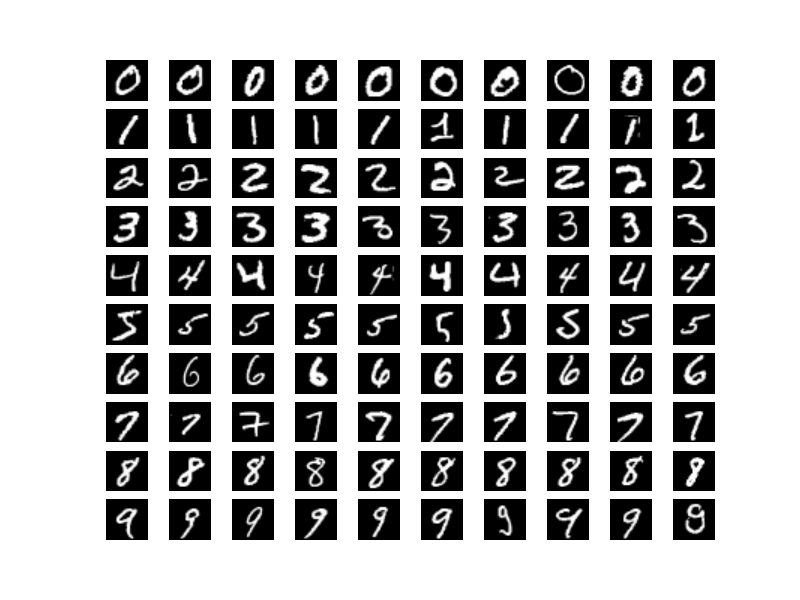
\includegraphics[width=0.95\linewidth]{part1.png}
\end{center}
\end{figure*}
\end{homeworkProblem}
\clearpage
%----------------------------------------------------------------------------------------
%	PART 2
%----------------------------------------------------------------------------------------
\begin{homeworkProblem}
\begin{lstlisting}[language=Python]
def softmax(y):
    '''Return the output of the softmax function for the matrix of output y. y
    is an NxM matrix where N is the number of pixels, and M is the number of samples'''
    return exp(y)/tile(sum(exp(y),0), (len(y),1))
    
def output(W, x):
    # Add 1 on top of x, this is for the bias b. 
    x = vstack((ones((1, x.shape[1])), x))
    o = dot(W.T, x)
    p = softmax(o)
    return o, p
\end{lstlisting}
\textbf{Note:} I added the bias b directly into the matrix calculation. The professor stated that it is acceptable @332 Piazza. \\
\end{homeworkProblem}


%----------------------------------------------------------------------------------------
%	PART 3
%----------------------------------------------------------------------------------------
\begin{homeworkProblem}
\textbf{Part A:} \\
We have the cost function as follows:
\begin{equation}
C = -\sum_i(y_ilog(p_i)) \\
\end{equation}
In which:
\begin{equation}
p_i = \dfrac{e^{o_i}}{\sum_ke^{o_k}} \\
\end{equation}
Let's compute $\dfrac{dp_i}{do_j}$ using the quotation rule.\\
\textbf{Case 1: } When $i \neq j$ 
\begin{equation}
\begin{split}
\dfrac{dp_i}{do_j} &= -\dfrac{e^{o_i} \times e^{o_j}}{(\sum_ke^{o_k})^2} \\
& = -p_ip_j
\end{split}
\end{equation}
\textbf{Case 2:} When $i = j$
\begin{equation}
\begin{split}
\dfrac{dp_i}{do_j} &= \dfrac{e^{o_i}(\sum_ke^{o_k}) - e^{o_i}e^{o_i}}{(\sum_ke^{o_k})^2} \\
& = \dfrac{e^{o_i} ((\sum_ke^{o_k}) - e^{o_i}))}{(\sum_ke^{o_k})(\sum_ke^{o_k})} \\
&= \dfrac{e^{o_i}}{\sum_ke^{o_k}} \times (1 - \dfrac{e^{o_i}}{\sum_ke^{o_k}}) \\
&= p_i - (1 - p_i) \\
&= p_j - (1 - p_j)
\end{split}
\end{equation}
We want $\dfrac{dC}{do_j} = \dfrac{dC}{dp_i} \times \dfrac{dp_i}{do_j}$. 
\begin{equation}
\begin{split}
\dfrac{dC}{do_j} &= -\sum_i(y_i\dfrac{d}{do_j}log(p_i)) \\
&= -\sum_i(y_i\dfrac{d}{p_i}log(p_i)\times\dfrac{dp_i}{do_j}) \\
&= -\sum_i(\dfrac{y_i}{p_i}\times\dfrac{dp_i}{do_j}) \\
&= -(\dfrac{y_j}{p_j}p_j(1-p_j) + \sum_{i \neq j}(\dfrac{y_i}{p_i}\times\dfrac{dp_i}{do_j})) \\
&= -(y_j(1-p_j) + \sum_{i \neq j}(\dfrac{y_i}{p_i}\times\dfrac{dp_i}{do_j})) \\
&= -(y_j-y_jp_j + \sum_{i \neq j}(\dfrac{y_i}{p_i}\times -(p_ip_j))) \\
&= -(y_j-y_jp_j - \sum_{i \neq j}(y_ip_j)) \\
&= -(y_j - \sum_{i}(y_ip_j)) \\
&= -(y_j - p_j\sum_{i}(y_i))\\
&= -(y_j - p_j \times 1) \qquad Only \ one \  1  \ in  \ y.\\
&= p_j - y_j
\end{split}
\end{equation}
We have $do_{j} = \sum_iw_{i, j}x_i + b_j$, then $\dfrac{do_{j}}{dw_{i, j}} = x_i$. Again, we apply the chain rule to get the final deriative: \\
\begin{equation}
\begin{split}
\dfrac{dC}{dW_{i, j}} &= \dfrac{dC}{do_j} \times \dfrac{do_{j}}{dw_{i, j}} \\
&= x_i (p_j-o_j)
\end{split}
\end{equation}
That is for a single sample. Let m be the size of the training set, then, the gradient with respect to $W_{i,j}$ is: \\
\begin{equation}
\sum^m_k(x_i^{(k)}(p_j^{(k)} - o_j^{(k)}))
\end{equation}
You can run the code in \textit{digits.py}, to verify this result agaist the vectorized gradient function.

\textbf{Part B}
\begin{lstlisting}
def compute_p_part3(W,x):
    o = dot(W.T, x)
    p = softmax(o)
    return o, p

# Vectorized gradient function.
def vectorized_gradient_part3(x, y, W):
    x = vstack((ones((1, x.shape[1])), x))
    return dot(x, (compute_p_part3(W, x)[1] - y).T)
\end{lstlisting}
\textbf{Note: } This is almost identical to the vectorized gradient in assignment 1.
\end{homeworkProblem}


%----------------------------------------------------------------------------------------
%	PART 4
%----------------------------------------------------------------------------------------
\begin{homeworkProblem}
\textbf{Step size $\alpha = 10^{-11}$ } \\
\textbf{Initial weight $w_{initial}=0$ } \\\\
Like in linear regression, I need a step size $\alpha$ that is neither too big or too small. $\alpha$ should not be too small, because it would take too many iterations for gradient descent to reach the local minimum. Else if $\alpha$ is too big, the algorithm could miss the local optimal point, and diverge to infinity, causing numerical overflow. $\alpha = 10^{-11}$ was the result of a trial and error process. This alpha level allowed me to construct a smooth learning curve and produced nice visualizations of the $weights$, which I could not get with the lower values. I also need an intital $weight_{initial}$, which is sufficiantly small to run gradient descent. To keep it simple, I set the  $weight_{initial}$ to be a vector with only zeros. \\\\
\textbf{Visualization of the $weights$} 
\begin{figure*}[!ht]
\begin{subfigure}{.33\textwidth}
\begin{center}
  
\includegraphics[width=.35\linewidth]{part4_img_0.png}
  \caption{0}
  \label{fig:sfig1}
\end{center}
\end{subfigure}
\begin{subfigure}{.33\textwidth}
\begin{center}
  
\includegraphics[width=.35\linewidth]{part4_img_1.png}
  \caption{1}
  \label{fig:sfig2}
\end{center}
\end{subfigure}
\begin{subfigure}{.33\textwidth}
\begin{center}
  
\includegraphics[width=.35\linewidth]{part4_img_2.png}
  \caption{2}
  \label{fig:sfig3}
\end{center}
\end{subfigure}
\begin{subfigure}{.33\textwidth}
\begin{center}
  
\includegraphics[width=.35\linewidth]{part4_img_3.png}
  \caption{3}
  \label{fig:sfig4}
\end{center}
\end{subfigure}
\begin{subfigure}{.33\textwidth}
\begin{center}
  
\includegraphics[width=.35\linewidth]{part4_img_4.png}
  \caption{4}
  \label{fig:sfig5}
\end{center}
\end{subfigure}
\begin{subfigure}{.33\textwidth}
\begin{center}
  
\includegraphics[width=.35\linewidth]{part4_img_5.png}
  \caption{5}
  \label{fig:sfig6}
\end{center}
\end{subfigure}
\begin{subfigure}{.33\textwidth}
\begin{center}
  
\includegraphics[width=.35\linewidth]{part4_img_6.png}
  \caption{6}
  \label{fig:sfig4}
\end{center}
\end{subfigure}
\begin{subfigure}{.33\textwidth}
\begin{center}
  
\includegraphics[width=.35\linewidth]{part4_img_7.png}
  \caption{7}
  \label{fig:sfig5}
\end{center}
\end{subfigure}
\begin{subfigure}{.33\textwidth}
\begin{center}
  
\includegraphics[width=.35\linewidth]{part4_img_8.png}
  \caption{8}
  \label{fig:sfig6}
\end{center}
\end{subfigure}
\begin{subfigure}{.33\textwidth}
\begin{center}
  
\includegraphics[width=.35\linewidth]{part4_img_9.png}
  \caption{9}
  \label{fig:sfig6}
\end{center}
\end{subfigure}
\caption{}
\end{figure*}
\clearpage
\textbf{Learning curve:}
\begin{figure*}[!ht]
\begin{center}
  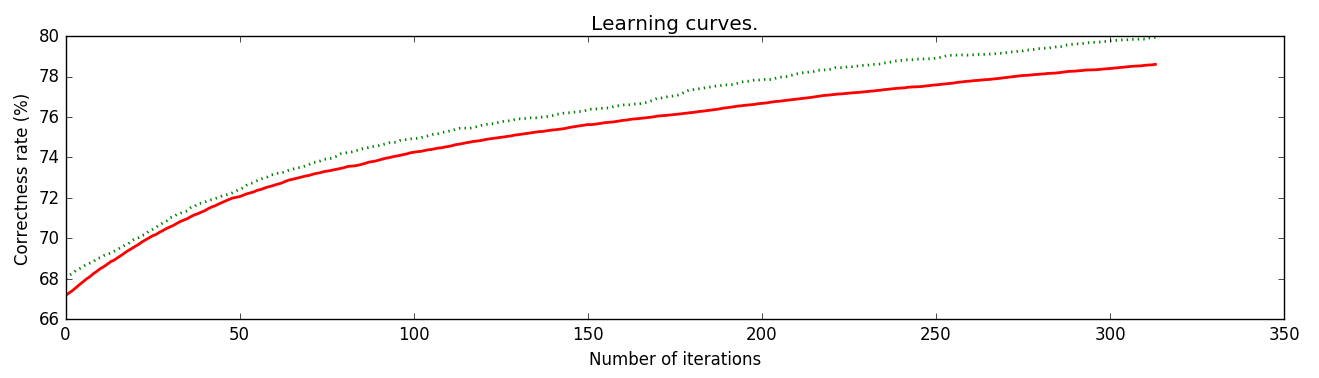
\includegraphics[width=.9\linewidth]{part4_plot.png}
  \caption{Learning curve: red line represents for the performance on the taining set. Green dotted line represents the performance on the testing set.}
\end{center}
\end{figure*}
\end{homeworkProblem}


%----------------------------------------------------------------------------------------
%	PART 5
%----------------------------------------------------------------------------------------
\begin{homeworkProblem}
Generate a training sample of size 200, that has normal distribution $N(\bar{x}=0, \sigma^2 = 0.1)$
\begin{lstlisting}[language=Python]
def part5():
    m = 200
    n = 2 # number of feature + 1
    k = 2 # number of possible labels
    
    # Training data
    np.random.seed(1)
    mu, sigma = 0, 0.1 # mean and standard deviation.
    s = np.random.normal(mu, sigma, m)
    s = s.reshape((1,m))
        
    print("------- Training data with no outlier -------")
    print(s)
\end{lstlisting}
Because of the small variance, the data points are all around 0. Below is the set of 200 data points that gets printed. Note that the first element in this array will be replaced by an outlier. 
\begin{lstlisting}[language=Python]
[[ 0.16243454 -0.06117564 -0.05281718 -0.10729686  0.08654076 -0.23015387
   0.17448118 -0.07612069  0.03190391 -0.02493704  0.14621079 -0.20601407
  -0.03224172 -0.03840544  0.11337694 -0.10998913 -0.01724282 -0.08778584
   0.00422137  0.05828152 -0.11006192  0.11447237  0.09015907  0.05024943
   0.09008559 -0.06837279 -0.01228902 -0.09357694 -0.02678881  0.05303555
  -0.06916608 -0.03967535 -0.06871727 -0.08452056 -0.06712461 -0.00126646
  -0.11173103  0.02344157  0.16598022  0.07420442 -0.01918356 -0.0887629
  -0.07471583  0.16924546  0.00508078 -0.06369956  0.01909155  0.21002551
   0.0120159   0.06172031  0.03001703 -0.03522498 -0.11425182 -0.03493427
  -0.02088942  0.05866232  0.08389834  0.09311021  0.02855873  0.08851412
  -0.07543979  0.12528682  0.05129298 -0.02980928  0.04885181 -0.00755717
   0.11316294  0.15198168  0.21855754 -0.13964963 -0.14441138 -0.05044659
   0.01600371  0.08761689  0.03156349 -0.20222012 -0.0306204   0.08279746
   0.02300947  0.07620112 -0.02223281 -0.02007581  0.01865614  0.04100516
   0.01982997  0.01190086 -0.06706623  0.03775638  0.01218213  0.11294839
   0.11989179  0.01851564 -0.0375285  -0.06387304  0.04234944  0.00773401
  -0.03438537  0.00435969 -0.06200008  0.0698032  -0.04471286  0.12245077
   0.04034916  0.05935785 -0.10949118  0.01693824  0.07405565 -0.09537006
  -0.02662185  0.00326145 -0.13731173  0.03151594  0.08461606 -0.08595159
   0.0350546  -0.13122834 -0.00386955 -0.16157724  0.11214177  0.04089005
  -0.0024617  -0.07751616  0.12737559  0.19671017 -0.18579819  0.1236164
   0.16276508  0.03380117 -0.1199268   0.08633453 -0.01809203 -0.06039206
  -0.12300581  0.05505375  0.07928069 -0.06235307  0.05205763 -0.11443414
   0.0801861   0.00465673 -0.01865698 -0.01017459  0.08688862  0.07504116
   0.05294653  0.01377012  0.00778211  0.06183803  0.02324946  0.06825514
  -0.03101168 -0.24348378  0.10388246  0.21869796  0.04413644 -0.01001552
  -0.01364447 -0.01190542  0.00174094 -0.11220187 -0.05170945 -0.09970268
   0.02487992 -0.02966412  0.04952113 -0.01747032  0.09863352  0.02135339
   0.21906997 -0.18963609 -0.06469167  0.09014869  0.25283257 -0.02486348
   0.0043669  -0.02263142  0.13314571 -0.02873079  0.06800698 -0.03198016
  -0.12725588  0.03135477  0.05031848  0.12932259 -0.0110447  -0.06173621
   0.05627611  0.02407371  0.02806651 -0.00731127  0.11603386  0.03694927
   0.19046587  0.11110567  0.06590498 -0.16274383  0.06023193  0.04202822
   0.08109517  0.10444421]]
\end{lstlisting}
I do the classification on these data, all data points less than 0 are labelled 0 and other data points greater than 0 are labelled 1. The fun thing is I will change the first element in the array to be a very large number, that will definitely make big impact on the cost function as well as the gradient produced by the gradient descent algorithm. 
\begin{lstlisting}[language=Python]
    # classification
    y = zeros((k, m))
    for i in range(m):
        if s[0][i] > 0:
            y[1][i]= 1;
        elif s[0][i] <= 0:
            y[0][i] = 1;
    
    # Let put an outlier into s.
    s[0][0] = 50000;
\end{lstlisting} 
The very first element is now set to 50000, a value that is far away from the sample mean 0. I will run both linear and logistic regression on the data, and print the performance.
\begin{lstlisting}[language=Python]
    init_theta = np.zeros((n, k)) # each sample has only 1 feature + 1 for the bias.
    alpha = 0.000000000001
    
    # Linear gradient descent.
    theta = grad_descent_linear_part5(s, y, init_theta, alpha)
    # Logistic graident descent.
    weight = grad_descent_logistic_part5(s, y, init_theta, alpha)
    
    # Linear regression result on training data.
    linear_result = (dot(theta[1:].T, s) + theta[0].reshape(k,1))
    
    # Logistic regression on training data
    logistic_result = (dot(weight[1:].T, s) + weight[0].reshape(k,1))
    
    correct_count_linear = 0;
    corect_count_logistic = 0;
    
    y = y.T
    linear_result = linear_result.T
    logistic_result = logistic_result.T
    
    for i in range(m):
        if (argmax(y[i]) == argmax(linear_result[i])):
            correct_count_linear = correct_count_linear + 1;
        if (argmax(y[i]) == argmax(logistic_result[i])):
            corect_count_logistic = corect_count_logistic + 1;
    
    print("------- Performance report on training data -------")
    print("Linear regression on training set with the outlier.",
     float(correct_count_linear)/float(len(y)) * 100)
    print("Logistic to regression on training set with the outlier.",
     float(corect_count_logistic)/float(len(y)) * 100)
\end{lstlisting} 
Below is the performance on the training data reported by the program.
\begin{lstlisting}[language=Python]
------- Performance report on training data -------
('Linear regression on training set with the outlier.', 63.5)
('Logistic regression on training set with the outlier.', 96.5)
\end{lstlisting} 
The correctness rate on the training set using logistic regression is $96.5\%$, whereas the corretness rate for linear regression is only $63.5\%$. The difference is due to the cost function $C=\sum_i(\sum_j(\theta^Tx^{(i)} - y^{(i)})_j^{2})$ of linear regression is heavily impacted by the outlier value 50000. If you make the outlier value larger, the performance of linear regression will get even worse. \\
I create a test set with the same sample size, same sample distribution, but with no outlier.
\begin{lstlisting}[language=Python]
    np.random.seed(3)
    
    test_data = np.random.normal(mu, sigma, m)
    test_data = test_data.reshape((1, m))
    
    print("------- Test data with no outlier. -------")
    print(test_data)  
    
    # Classification of the test data.
    y_test = zeros((k, m))
    for i in range(m):
        if test_data[0][i] > 0:
            y_test[1][i]= 1;
        elif test_data[0][i] <= 0:
            y_test[0][i] = 1;
            
    linear_result_test = (dot(theta[1:].T, test_data) + theta[0].reshape(k,1))
    logistic_result_test = (dot(weight[1:].T, test_data) + weight[0].reshape(k,1))
    
    y_test = y_test.T
    linear_result_test = linear_result_test.T
    logistic_result_test = logistic_result_test.T
    
    correct_count_linear = 0;
    corect_count_logistic = 0;
    for i in range(m):
        if (argmax(y_test[i]) == argmax(linear_result_test[i])):
            correct_count_linear = correct_count_linear + 1;
        if (argmax(y_test[i]) == argmax(logistic_result_test[i])):
            corect_count_logistic = corect_count_logistic + 1;
            
    print("------- Performance report on training data -------")
    print("Linear regression on test set", 
    float(correct_count_linear)/float(len(y)) * 100)
    print("Logistic to regression on test set", 
    float(corect_count_logistic)/float(len(y)) * 100)
\end{lstlisting} 
Below is the performance report on the testing data. As expected, the performance using logistic regression is still better. In conclusion, if you have a dataset with outliers that are much larger than other values, you better use logistic regression, as it is less impacted by the magnitude of the data.
\begin{lstlisting}[language=Python]
------- Performance report on training data -------
('Linear regression on test set', 56.49999999999999)
('Logistic to regression on test set', 96.0)
\end{lstlisting} 
\end{homeworkProblem}
\clearpage

%----------------------------------------------------------------------------------------
%	PART 6
%----------------------------------------------------------------------------------------
\begin{homeworkProblem}
Assuming that we have a fully connected $n \times n = 4 \times 4$ neural network with the following layout: \\
Layer 4: $l_{4,1}$  $l_{4,2}$  $l_{4,3}$  $l_{4,4}$ \\
Layer 3: $l_{3,1}$  $l_{3,2}$  $l_{3,3}$  $l_{3,4}$ \\
Layer 2: $l_{2,1}$  $l_{2,2}$  $l_{2,3}$  $l_{2,4}$ \\
Layer 1: $l_{1,1}$  $l_{1,2}$  $l_{1,3}$  $l_{1,4}$ \\
Each neuron in the network is a linear combination of all neurons in the layer right below it.\\
Let compute the deriative of the cost with respect every weight that connect layer 1 to layer 2. That is computing $\dfrac{dC}{dW_{1,i,j}}$ for every possible $i$ and $j$. $W_{1,i,j}$ is a component of the weight matrix that connects the neuron i in layer 1 to the neuron j in layer 2.\\
\textbf{1. Weights connect $l_{1,1}$ in layer 1 to all nodes in layer2.}\\
\setcounter{equation}{0}
\begin{equation}
\begin{split}
\dfrac{dC}{dW_{1,1,1}} &= \dfrac{dC}{dl_{2,1}} \times \dfrac{dl_{2,1}}{dW_{1,1,1}} \\
\dfrac{dC}{dl_{2,1}} &= \sum_k^n \dfrac{dC}{dl_{3,k}} \times \dfrac{dl_{3,k}}{dl_{2,1}} \\
\dfrac{dC}{dl_{3,k}} &= \sum_i^n \dfrac{dC}{dl_{4,i}} \times \dfrac{dl_{4,i}}{dl_{3,k}} \\
\end{split}
\end{equation} \\
\begin{equation}
\begin{split}
\dfrac{dC}{dW_{1,1,2}} &= \dfrac{dC}{dl_{2,2}} \times \dfrac{dl_{2,2}}{dW_{1,1,2}} \\
\dfrac{dC}{dl_{2,2}} &= \sum_k^n \dfrac{dC}{dl_{3,k}} \times \dfrac{dl_{3,k}}{dl_{2,2}} \\
\dfrac{dC}{dl_{3,k}} &= \sum_i^n \dfrac{dC}{dl_{4,i}} \times \dfrac{dl_{4,i}}{dl_{3,k}} \\
\end{split}
\end{equation} \\
Note that we already computed $\{\dfrac{dC}{dl_{3,k}} | 0 \leq i \leq n \}$ in (1), so we can reuse them in (2). Let assume that $\dfrac{dC}{dl_{3,k}}$ costs $\theta(n)$ due to the n iterations of the summation $\sum_i^n \dfrac{dC}{dl_{4,i}} \times \dfrac{dl_{4,i}}{dl_{3,k}}$. Then by reusing the derivatives $\{ \dfrac{dC}{dl_{3,k}} | 0 \leq i \leq n \}$ already computed in (1), we save $\theta(n \times n) = \theta(n^2)$ units of time in the calculation of $\dfrac{dC}{dW_{1,1,2}}$.\\

We are also able to reuse $\{\dfrac{dC}{dl_{3,k}} | 0 \leq i \leq n \}$ in the calculations of $\dfrac{dC}{dW_{1,1,3}}$ and $\dfrac{dC}{dW_{1,1,4}}$. \\
\begin{equation}
\begin{split}
\dfrac{dC}{dW_{1,1,3}} &= \dfrac{dC}{dl_{2,3}} \times \dfrac{dl_{2,3}}{dW_{1,1,3}} \\
\dfrac{dC}{dl_{2,3}} &= \sum_k^n \dfrac{dC}{dl_{3,k}} \times \dfrac{dl_{3,k}}{dl_{2,3}} \\
\dfrac{dC}{dl_{3,k}} &= \sum_i^n \dfrac{dC}{dl_{4,i}} \times \dfrac{dl_{4,i}}{dl_{3,k}} \\
\end{split}
\end{equation} \\
\begin{equation}
\begin{split}
\dfrac{dC}{dW_{1,1,4}} &= \dfrac{dC}{dl_{2,4}} \times \dfrac{dl_{2,4}}{dW_{1,1,4}} \\
\dfrac{dC}{dl_{2,4}} &= \sum_k^n \dfrac{dC}{dl_{3,k}} \times \dfrac{dl_{3,k}}{dl_{2,4}} \\
\dfrac{dC}{dl_{3,k}} &= \sum_i^n \dfrac{dC}{dl_{4,i}} \times \dfrac{dl_{4,i}}{dl_{3,k}} \\
\end{split}
\end{equation} \\
At each of the computations of $\dfrac{dC}{dW_{1,1,2}}$, $\dfrac{dC}{dW_{1,1,3}}$, $\dfrac{dC}{dW_{1,1,4}}$ we saved $\theta(n^2)$ units of time, so overall we saved $3 \times \theta(n^2) = (n-1) \times \theta(n^2) = \theta (n^3)$ units of time. \\

\textbf{2. Weights connect $l_{1,2}$ in layer 1 to all nodes in layer2.}\\
\begin{equation}
\dfrac{dC}{dW_{1,2,1}} = \dfrac{dC}{dl_{2,1}} \times \dfrac{dl_{2,1}}{dW_{1,2,1}} \\
\end{equation}
\begin{equation}
\dfrac{dC}{dW_{1,2,2}} = \dfrac{dC}{dl_{2,2}} \times \dfrac{dl_{2,2}}{dW_{1,2,2}} \\
\end{equation}
\begin{equation}
\dfrac{dC}{dW_{1,2,3}} = \dfrac{dC}{dl_{2,3}} \times \dfrac{dl_{2,3}}{dW_{1,2,3}} \\
\end{equation}
\begin{equation}
\dfrac{dC}{dW_{1,2,4}} = \dfrac{dC}{dl_{2,4}} \times \dfrac{dl_{2,4}}{dW_{1,2,4}} \\
\end{equation}
$\dfrac{dC}{dl_{2,1}}$, $\dfrac{dC}{dl_{2,2}}$, $\dfrac{dC}{dl_{2,3}}$ and $\dfrac{dC}{dl_{2,4}}$ were computed in the first part, so we can basically reuse the answer and save another $\theta(n^3)$.\\
\textbf{3. Weights connect $l_{1,3}$ in layer 1 to all nodes in layer2.}\\
\begin{equation}
\dfrac{dC}{dW_{1,3,1}} = \dfrac{dC}{dl_{2,1}} \times \dfrac{dl_{2,1}}{dW_{1,3,1}} \\
\end{equation}
\begin{equation}
\dfrac{dC}{dW_{1,3,2}} = \dfrac{dC}{dl_{2,2}} \times \dfrac{dl_{2,2}}{dW_{1,3,2}} \\
\end{equation}
\begin{equation}
\dfrac{dC}{dW_{1,3,3}} = \dfrac{dC}{dl_{2,3}} \times \dfrac{dl_{2,3}}{dW_{1,3,3}} \\
\end{equation}
\begin{equation}
\dfrac{dC}{dW_{1,3,4}} = \dfrac{dC}{dl_{2,4}} \times \dfrac{dl_{2,4}}{dW_{1,3,4}} \\
\end{equation}
We continue reuse $\dfrac{dC}{dl_{2,1}}$, $\dfrac{dC}{dl_{2,2}}$, $\dfrac{dC}{dl_{2,3}}$ and $\dfrac{dC}{dl_{2,4}}$ to save $\theta(n^3)$ units of time. \\
\textbf{4. Weights connect $l_{1,4}$ in layer 1 to all nodes in layer2.}\\
\begin{equation}
\dfrac{dC}{dW_{1,4,1}} = \dfrac{dC}{dl_{2,1}} \times \dfrac{dl_{2,1}}{dW_{1,4,1}} \\
\end{equation}
\begin{equation}
\dfrac{dC}{dW_{1,4,2}} = \dfrac{dC}{dl_{2,2}} \times \dfrac{dl_{2,2}}{dW_{1,4,2}} \\
\end{equation}
\begin{equation}
\dfrac{dC}{dW_{1,4,3}} = \dfrac{dC}{dl_{2,3}} \times \dfrac{dl_{2,3}}{dW_{1,4,3}} \\
\end{equation}
\begin{equation}
\dfrac{dC}{dW_{1,4,4}} = \dfrac{dC}{dl_{2,4}} \times \dfrac{dl_{2,4}}{dW_{1,4,4}} \\
\end{equation}

Again, we are able reuse $\dfrac{dC}{dl_{2,1}}$, $\dfrac{dC}{dl_{2,2}}$, $\dfrac{dC}{dl_{2,3}}$ and $\dfrac{dC}{dl_{2,4}}$ from the first stage, so $\theta(n^3)$ more units of time can be saved. \\

If we sum the results, we get $TotalTime_{save} = \theta(n^3) + \theta(n^3) + \theta(n^3) + \theta(n^3) = 4\theta(n^3) = n\theta(n^3) = \theta(n^4) = \theta(n^n)$ units of time. \\

In general, if we have an $n \times n$ neural network, and we use back-propagation that "remember" the previous computed values, we will save $\theta(n^n)$ units of time. \\

\textbf{Note 1:} one of the key ideas in my explaination is that you can think of the summation $\sum$ as the for loop in the program, and the runtime of the summation is the number of iterations it makes. \\
\textbf{Note 2:} there are several interpretations of this question. I used the interpretation that has been confirmed by the professor at Piazza\@468. Below is the screenshot of the professor reply [1st answer].\\

\begin{figure*}[!ht]
\begin{center}
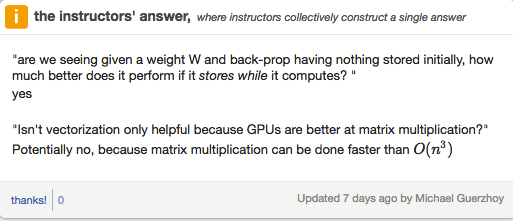
\includegraphics[width=.8\linewidth]{p6evidence.png}
\caption{Professor reply}
\end{center}
\end{figure*}
\end{homeworkProblem}
\clearpage

%----------------------------------------------------------------------------------------
%	PART 7
%----------------------------------------------------------------------------------------
\begin{homeworkProblem}
\textbf{Preprocessed the inputs:} I used the scipts \textit{get\_data\_and\_crop.py} to download the images of the 6 actors from the 2 tables of image URLs inside \textit{facescrub\_actors.txt} and \textit{facescrub\_actresses.txt}. For every image, the script computed its sha256 checksum and compared with the sha256 value given in the tables. Images failed the sha256 checksum were removed. \textit{get\_data\_and\_crop.py} put the downloaded images in the directory \textit{uncropped} and the cropped images in the directory \textit{cropped}. The cropped images are all grayscale of size $32x32$ pixels. All of the corrupted, bad images should had been removed vy sha256 checksum, but just to be sure I went over the images one more times, and removed few images that i thought were not good for classification purpose. Below are examples of images that I removed. \\\\
\begin{figure*}[!ht]
\begin{center}
\begin{subfigure}{.35\textwidth}
\begin{center}
  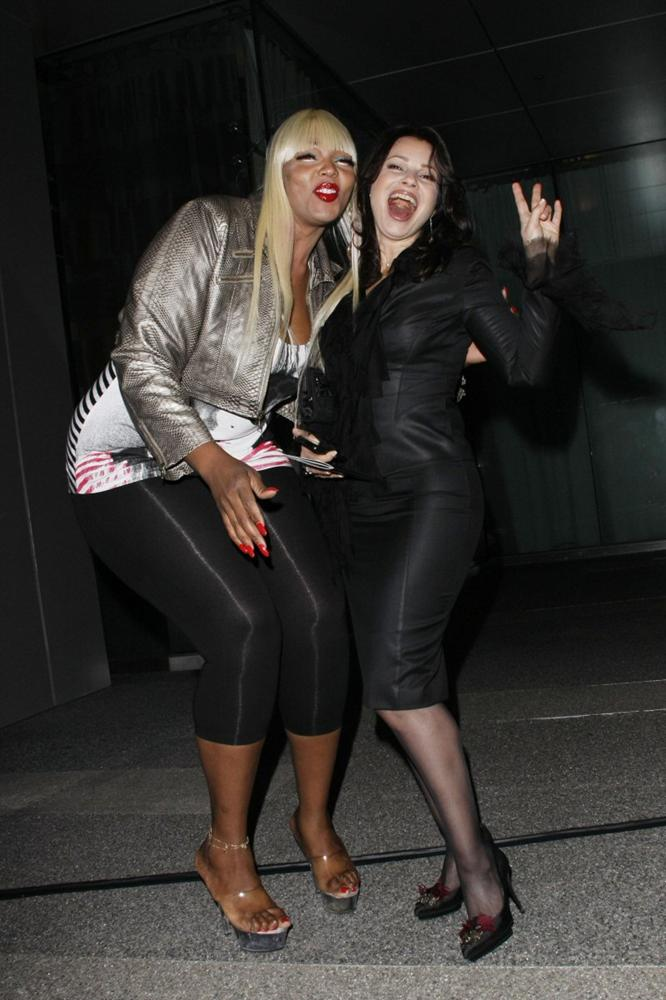
\includegraphics[width=.35\linewidth]{p7_drescher122.jpg}
  \label{fig:sfig3}
\end{center}
\caption{Original images}
\end{subfigure}
\begin{subfigure}{.4\textwidth}
\begin{center}
  
\includegraphics[width=.4\linewidth]{pp7_drescher122.jpg}
  \label{fig:sfig3}
\end{center}
\caption{Cropped images}
\end{subfigure}
\caption{Image with incorrect bounding box}
\end{center}
\end{figure*}

\begin{figure*}[!ht]
\begin{center}
\begin{subfigure}{.4\textwidth}
\begin{center}
  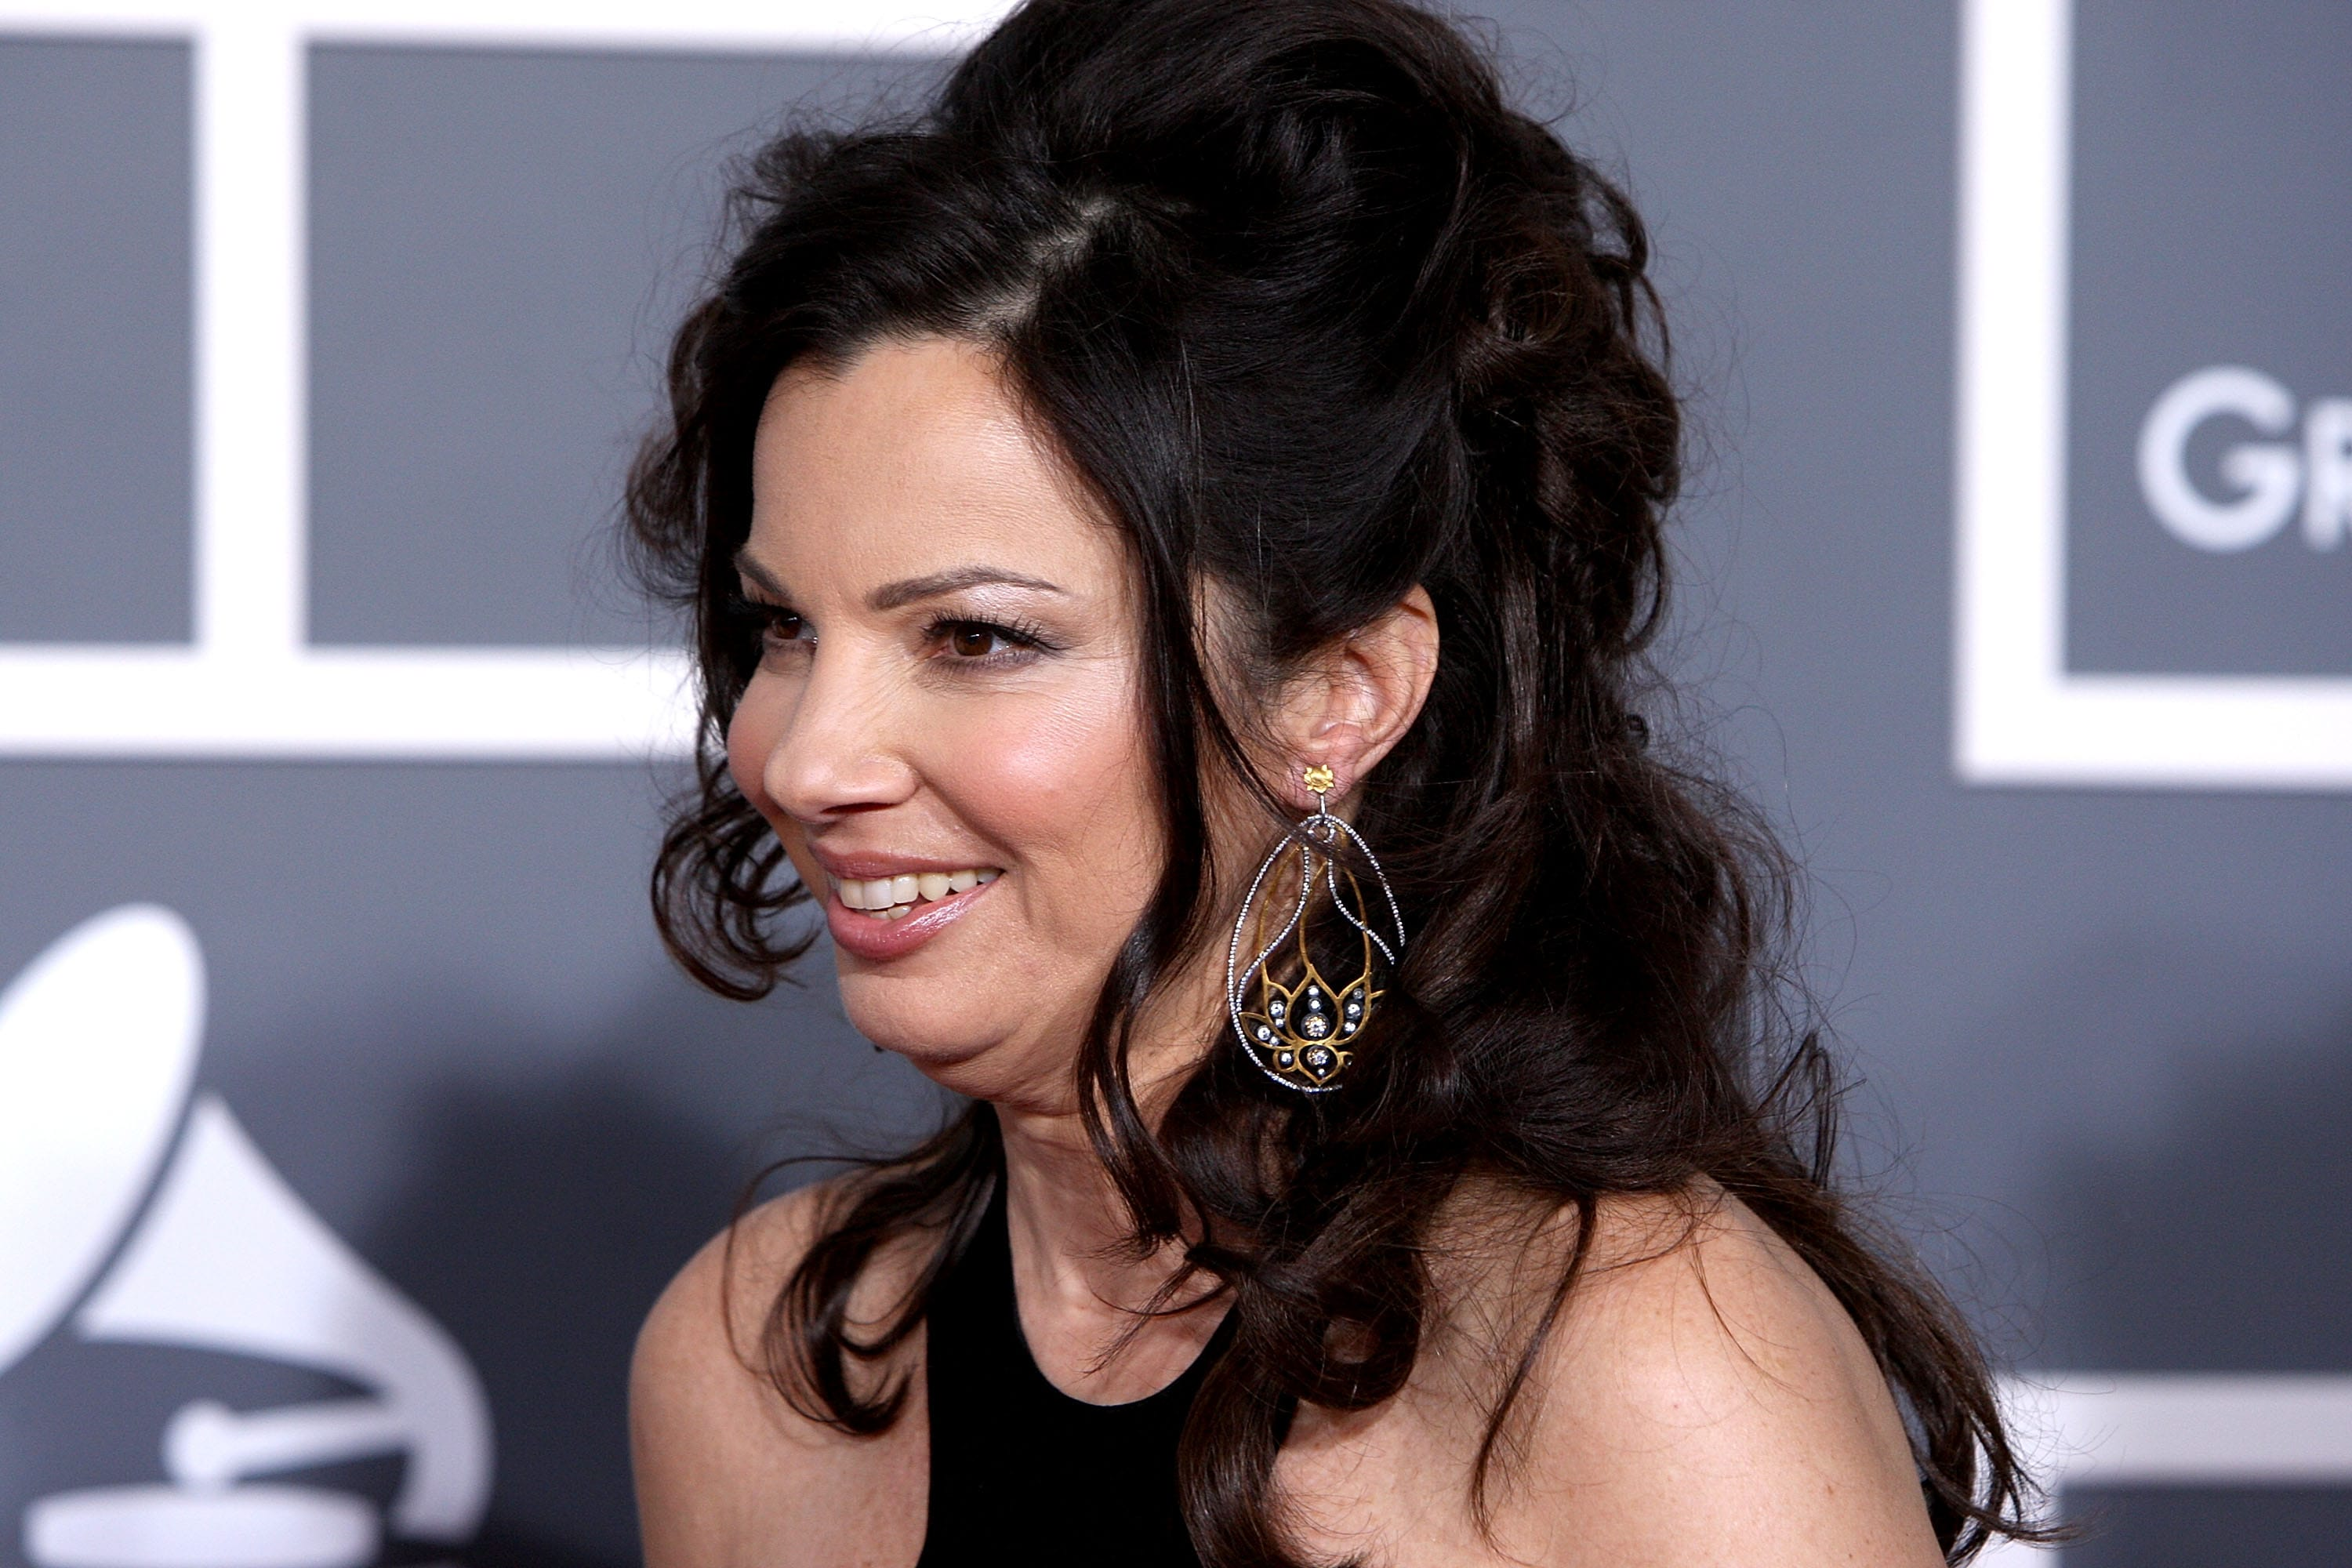
\includegraphics[width=.4\linewidth]{p7_drescher5.jpg}
\end{center}
\caption{Original images}
\end{subfigure}
\begin{subfigure}{.35\textwidth}
\begin{center}
  
\includegraphics[width=.35\linewidth]{pp7_drescher5.jpg}
\end{center}
\caption{Cropped images}
\end{subfigure}
\caption{Image shows only one side of the face}
\end{center}
\end{figure*} 

\begin{figure*}[!ht]
\begin{center}
\begin{subfigure}{.35\textwidth}
\begin{center}
  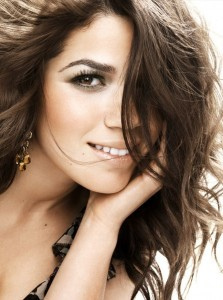
\includegraphics[width=.35\linewidth]{p7_ferrera165.jpg}
\end{center}
\caption{Original images}
\end{subfigure}
\begin{subfigure}{.35\textwidth}
\begin{center}
  
\includegraphics[width=.35\linewidth]{pp7_ferrera165.jpg}
\end{center}
\caption{Cropped images}
\end{subfigure}
\caption{Images show only one side of the face}
\end{center}
\end{figure*} 
\clearpage
\textbf{Picking training, validation and test set:} \\
I used the function \textit{def pickrandom()} in the script \textit{auto\_pick.py} to randomly pick 60 images for training, 30 images for validating and 30 images for testing. The three sets did not have any images in common. The script put the training images into \textit{part7\_data/train\_data}, validating images into \textit{part7\_data/valid\_data} and all testing images into \textit{part7\_data/test\_data}. \\\\
\textbf{Architecture of the network:} \\
It is a single-hidden-layer fully connected neuron network. There are 30 neurons in the hidden layer. The number of neuron in the input layer is corresponding to the number of pixels in an image which is $32*32=1024$ neurons. There are 6 possible outputs corresponding to the 6 actors, so the output layer has 6 neurons. \\\\
\textbf{Weight initialization:} \\
To run gradient descent, I need to initialize the weights for the edges that connect the input layer to the hidden layer as well as the edges that connect the hidden layer to the output layer. The weights were randomly generated usning normal distribution centralized at 0 with a small standard deviation of 0.01. Below are the codes used for initializing the weights. \\
\begin{lstlisting}[language=Python]
    W0 = tf.Variable(tf.random_normal([1024, nhid], stddev=0.01))
    b0 = tf.Variable(tf.random_normal([nhid], stddev=0.01))
    W1 = tf.Variable(tf.random_normal([nhid, 6], stddev=0.01))
    b1 = tf.Variable(tf.random_normal([6], stddev=0.01))
\end{lstlisting} 
\textbf{Activation function:}
I used the $tanh$ activation function for the network. I also tried with $Relu$ and $Sigmoid$, but none gave better performance than $tanh$ after 500 iterations of gradient descent. Below is the code illustration of how the activation can be applied. \\
\begin{lstlisting}[language=Python]
    layer1 = tf.nn.tanh(tf.matmul(x, W0)+b0)
    # layer1 = tf.nn.sigmoid(tf.matmul(x, W0)+b0)
    # layer1 = tf.nn.relu(tf.matmul(x, W0)+b0)
    layer2 = tf.matmul(layer1, W1)+b1
\end{lstlisting}
\textit{References: https://www.tensorflow.org/api\_guides/python/nn} \\
\clearpage
\textbf{Learning curves with 30 hidden units} 
\begin{figure*}[!ht]
\begin{center}
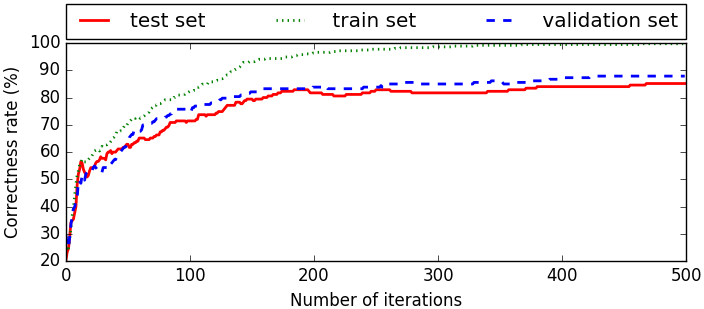
\includegraphics[width=.9\linewidth]{plot_part7_best.png}
\caption{The performance on the training set come very closed to 100\% after 500 iterations of gradient descent. The correctness rates on the validation and testing set are peaked at 87\%, this is the highest value that I could get after trying to vary the number of hidden units as well as using different activation functions. Any number of hidden units greater than 30 would not give better performance on the validation and testing set than this configuration.}
\end{center}
\end{figure*} \\
\textit{Note:} I recognized that there was a bit of overfitting since the performance on the traing set was 10 \% higher than the validation and test set, but there were no other configurations that could give me better testing and validating set performance than this one. \\\\
\textbf{Learning curves with only 5 hidden units} \\
\begin{figure*}[!ht]
\begin{center}
 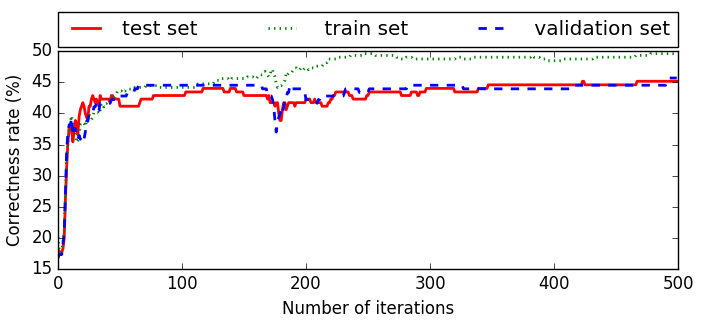
\includegraphics[width=.9\linewidth]{plot_part7_underfitting.png}
\caption{After 500 iterations, a neural network with only 5 hidden units only gave the correct rates no better than 50 \%. This is to illustrate that the number of hidden units in a network could influence the performance. In this case, the low number of hidden units caused underfitting.}
\end{center}
\end{figure*}
\end{homeworkProblem}
\clearpage


%----------------------------------------------------------------------------------------
%	PART 08
%----------------------------------------------------------------------------------------
\begin{homeworkProblem}
\textbf{Codes: } The codes for this part are in \textit{faces.py} and \textit{get\_data\_and\_crop.py}. \\
\textbf{Prepare Data:} Like in part 7, please use the script \textit{get\_data\_and\_crop.py} to download and crop the faces of the 6 actors. \\
\textbf{Overfitting Scenario:} To create an overfitting scenario for which I can demonstrate the use of weight decay, I do the followings:
\begin{itemize}
\item I have a small training set that consists only 48 images, 8 for each of the actors. The size of validation and test set are both $40 \times 6 = 280$, that is much larger than the training set. 
\item I use a single hidden layer network to do the classification. The hidden layer has 2000 units, which is almost twice the number of features $32 \times 32 = 1024$ (i.e. the pixels) in an image.
\item Recalling from class that small training test size and large number of hidden units are common reasons for overfitting.
\end{itemize}
\textbf{Strategy for testing: } \\
The function \textit{part8\_with\_no\_regularization()} is used compute the performance on the training, validation and test set without the use of weight decay. The function \textit{part8\_with\_regularization()} is used to compute the performance with the same sets, but with the use weight decay. \\
\textbf{Regularization codes:}
\begin{lstlisting}[language=Python]
    lam = 0.8
    decay_penalty = lam * tf.reduce_sum(tf.square(W0)) + lam * tf.reduce_sum(tf.square(W1))
    reg_NLL = -tf.reduce_sum(y_*tf.log(y)) + decay_penalty
\end{lstlisting}
With the $\lambda$ for weight decay set to 0.8, the performances on both validation and test set are improved. I chose the lamda based on how much improvement was made on the validation set with the use of weight decay.

\textbf{Comparision results}: Below are the results obtained from different runs of  \textit{part8\_with\_no\_regularization()} and \textit{part8\_with\_regularization()}. Even though the improvement is only 2 to 6 \%, it is significant because we have a fairly large validation and testing sets. 
\begin{lstlisting}[language=Python]
	## ========= RUN 1 ========= ##	
	-----With no regularization------
	('Performance on the test set: ', 0.80000001)
	('Performance on the train set: ', 1.0)
	('Performance on the validation set:', 0.82080925)

	-----With-regularization------
	('Performance on the test set: ', 0.81142855)
	('Performance on the train set: ', 0.99430197)
	('Performance on the validation set:', 0.84393066)
	
	## ========= RUN 2 ========= ##
	-----With no regularization------
	('Performance on the test set: ', 0.81714284)
	('Performance on the train set: ', 1.0)
	('Performance on the validation set:', 0.79768789)

	-----With-regularization------
	('Performance on the test set: ', 0.81714284)
	('Performance on the train set: ', 0.99715102)
	('Performance on the validation set:', 0.82080925)
	
	## ========= RUN 3 ========= ##
	-----With no regularization------
	('Performance on the test set: ', 0.81142855)
	('Performance on the train set: ', 0.99715102)
	('Performance on the validation set:', 0.79768789)

	-----With-regularization------
	('Performance on the test set: ', 0.81714284)
	('Performance on the train set: ', 0.99430197)
	('Performance on the validation set:', 0.83236992)
\end{lstlisting}
\end{homeworkProblem}
\clearpage

%----------------------------------------------------------------------------------------
%	PART 09
%----------------------------------------------------------------------------------------
\begin{homeworkProblem}
\textbf{Codes:} The codes for this part are in \textit{faces.py}  \\
\textbf{Selecting hidden units:} From part 7, we have a single hidden layer network with W0 and W1. W0 is a weight matrix vector of size $1024 \times 40$, in which $1024$ is the number of pixels of an image and $40$ is the number of hidden units. W0 connects the input layers to the hidden layer. W1 is a weight matrix of size $40 \times 6$, in which 40 is the number of hiddens units and 6 is the number of possible labels. \\\\
\textbf{Step 1:} I first find the 6 sensitive neurons, by looking at the $40 \times 6$ W1 weight matrix. The sensitive neurons are those that have high outgoing weight components. \\

\begin{lstlisting}[language=Python]
    #  40 * 6
    W1 = sess.run(W1, feed_dict={x: xs, y_: ys})
    # 6 * 40
    W1 = W1.T
    # Step 1: Find 6 hiddens unit that are most sensitive.
    unit = zeros(6)
    unit[0] = argmax(W1[0])
    unit[1] = argmax(W1[1])
    unit[2] = argmax(W1[2])
    unit[3] = argmax(W1[3])
    unit[4] = argmax(W1[4])
    unit[5] = argmax(W1[5])
\end{lstlisting}

\textbf{Step 2:} I then extract the incoming weights to the sensitive neurons from W0, and dislay only these weights. 
\begin{lstlisting}[language=Python]
    # 1024 * nhid = 1024 * 40
    W0 = sess.run(W0, feed_dict={x: xs, y_: ys})
    # 40 * 1024
    W0 = W0.T
    # Step 2: Extract 6 weights come into the 6 sensitive neurons.
    img0 = imresize((W0[unit[0]]).reshape(32, 32), (64, 64))
    img1 = imresize((W0[unit[1]]).reshape(32, 32), (64, 64))
    img2 = imresize((W0[unit[2]]).reshape(32, 32), (64, 64))
    img3 = imresize((W0[unit[3]]).reshape(32, 32), (64, 64))
    img4 = imresize((W0[unit[4]]).reshape(32, 32), (64, 64))
    img5 = imresize((W0[unit[5]]).reshape(32, 32), (64, 64))
  	
  	# Save images to local folder.
    imsave("part9_img0.png", img0)
    imsave("part9_img1.png", img1)
    imsave("part9_img2.png", img2)    
    imsave("part9_img3.png", img3)
    imsave("part9_img4.png", img4)
    imsave("part9_img5.png", img5)
\end{lstlisting}
This strategy was confirmed by the Professor during the office hours as well as on Piazza @472. \\
For better resolution, I resize the images from $32 \times 32$ to $64 \times 64$ before saving the image to local directory. Out of the 6 images, I choose the best 3 to include in this report. Below are the images:\\\\

\begin{figure*}[!ht]
\begin{center}
\begin{subfigure}{.55\textwidth}
\begin{center}
  
\includegraphics[width=.55\linewidth]{part9_img1.png}
\end{center}
\caption{}
\end{subfigure}
\begin{subfigure}{.55\textwidth}
\begin{center}
  
\includegraphics[width=.55\linewidth]{part9_img2.png}
\end{center}
\caption{}
\end{subfigure}
\begin{subfigure}{.55\textwidth}
\begin{center}
  
\includegraphics[width=.55\linewidth]{part9_img5.png}
\end{center}
\caption{}
\end{subfigure}
\caption{To make the images look smoother, I also used weight decay with $\lambda=10$.}
\end{center}
\end{figure*} 
\end{homeworkProblem}
\clearpage


%----------------------------------------------------------------------------------------
%	PART 10
%----------------------------------------------------------------------------------------
\begin{homeworkProblem}
\textbf{Codes: } The codes for this part is in \textit{get\_data\_and\_crop\_part10.py} and \textit{deepfaces.py}. \\

\textbf{Getting the data: } \\
The script \textit{get\_data\_and\_crop\_part10} was used to download the images for this part. The cropped face images for this part have size $227 \times 227$, not $32 \times 32$ like in part 7 or A1. \\

\textbf{Extract activations of AlexNet:} \\
To extract the values of activations, I input the $227 \times 227$ cropped face image into AlexNet, and grap the $13 \times 13 \times 384$ matrix returned at \textit{conv4}. The matrix can be thought as a set of features of a person image, and can be used for classification. \\

\textbf{Doing the classification:} \\
I build a single hidden layer network that is completely separated from the AlexNet. It takes in the extracted activations from \textit{conv4} of the cropped face images to do the training. \\

\textbf{Learning curves:} \\
\begin{figure*}[!ht]
\begin{center}
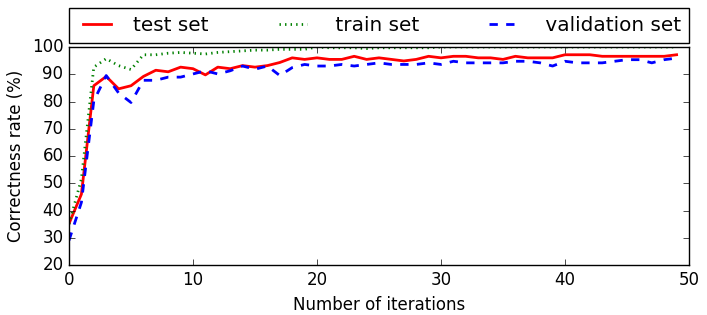
\includegraphics[width=.9\linewidth]{plot_part10.png}
\caption{After just 50 iterations, the correctness rates on the training, validation and testing sets are all greater than 95\%. }
\end{center}
\end{figure*} 

This is a big improvement on the performance when comparing to what we got in part 7. In part 7, we did 500 iterations, but if we only counted the first 50 iterations, none of the 3 sets has higher performance than 70\%. In conclusion, studying from features of the images is better than studying the images directly. \\
\end{homeworkProblem}
\clearpage
\end{document}